\documentclass[11pt]{article}

\usepackage[utf8]{inputenc} % Character encoding
\usepackage[T1]{fontenc}    % Large font encoding
\usepackage{lmodern}        % Latin modern font

\usepackage{float}
\usepackage{graphicx}
\usepackage{hyperref}

\usepackage{listings}	   % Code insertion
\lstdefinestyle{customstyle}{
    basicstyle=\footnotesize,
    breakatwhitespace=false,         
    breaklines=true,                 
    captionpos=b,                    
    keepspaces=true,                                                                                       
    tabsize=4,
    frame=single
}
\lstset{style=customstyle}	

\title{Projet Système de feux tricolores}
\author{Adrien Garandel \and Bao Ran \and Franck Boncler \and Jérémy Bardon}

\begin{document}

\maketitle
\tableofcontents
\newpage

%%%%%%%%%%%%%%%%%%%%%%%%%%%%%%%%%%%%%%%%%%%%
\section{Partie 1 - Deux feux synchronisés}
%%%%%%%%%%%%%%%%%%%%%%%%%%%%%%%%%%%%%%%%%%%%
Deux feux synchronisés mais non temporises

%%%%%%%%%%%%%%%%%%%%%%%
\subsection{Questions 1 et 2}
%%%%%%%%%%%%%%%%%%%%%%%

\href{https://github.com/masters-info-nantes/hong-cheng-lv/blob/master/ressources/part1/Q2-FeuxNonSynchro.xml}{Feux non synchronisés et non temporises}

\begin{figure}[H]
	\centering
	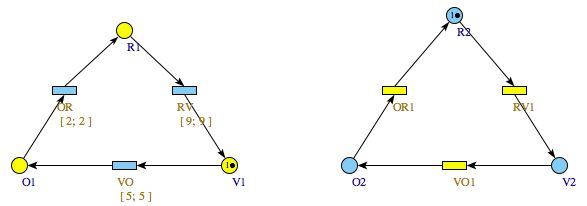
\includegraphics[width=1\textwidth]{ressources/part1/Q2.png}
	\caption{Réseau de Pétri, feux non synchronisés}
\end{figure}

%%%%%%%%%%%%%%%%%%%%%%%
\subsection{Question 3}
%%%%%%%%%%%%%%%%%%%%%%%

\href{https://github.com/masters-info-nantes/hong-cheng-lv/blob/master/ressources/part1/Q3-FeuxSynchro.xml}{Feux
synchronisés et non temporises}

\begin{figure}[H]
	\centering
	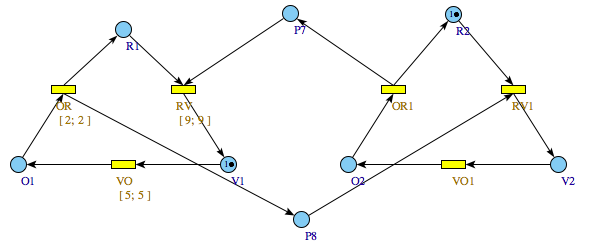
\includegraphics[width=1\textwidth]{ressources/part1/Q3.png}
	\caption{Réseau de Pétri, feux synchronisés}
\end{figure}

%%%%%%%%%%%%%%%%%%%%%%%
\subsection{Question 4}
%%%%%%%%%%%%%%%%%%%%%%%

\href{https://github.com/masters-info-nantes/hong-cheng-lv/blob/master/ressources/part1/Q4-GrapheMarquage.txt}{Graphe de marquage}

\begin{figure}[H]
	\centering
	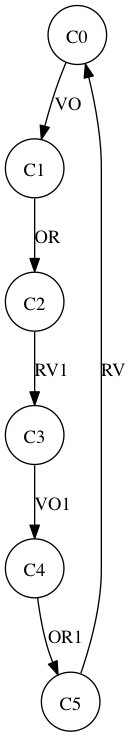
\includegraphics[scale=0.5]{ressources/part1/traitement-question4/graphe.png}
	\caption{Graphe de marquage des feux synchronisés}
\end{figure}

%%%%%%%%%%%%%%%%%%%%%%%
\subsection{Question 5}
%%%%%%%%%%%%%%%%%%%%%%%
Vérifications en LTL

%%%%%%%%%%%%%%%%%%%%%%%
\subsection{Question 6}
%%%%%%%%%%%%%%%%%%%%%%%

%%%%%%%%%%%
\subsubsection{Vérifications}
%%%%%%%%%%%

\textbf{Pas de 2 feux rouges en même temps (sureté)}
\begin{verbatim}
AG[0, inf](M(R1) + M(R2) >= 1)	
\end{verbatim}

\textbf{Un feu passe au moins une fois au vert (non bloqué)}
\begin{verbatim}
AG[0, inf](M(V2) = 1)	
\end{verbatim}
	
\textbf{Les feux ne se bloquent pas entre eux}
\begin{verbatim}
AG[0, inf](M(R1) + M(P7)) # P7 = place intermédiaire	
\end{verbatim}

%%%%%%%%%%%%%%%%%%%%%%%%%%%%%%%%%%%%%%%%%%%%
\section{Partie 2 - Deux feux temporises}
%%%%%%%%%%%%%%%%%%%%%%%%%%%%%%%%%%%%%%%%%%%%

%%%%%%%%%%%%%%%%%%%%%%%
\subsection{Question 7}
%%%%%%%%%%%%%%%%%%%%%%%

\href{https://github.com/masters-info-nantes/hong-cheng-lv/blob/master/ressources/part2/Q7-FeuxTemporises.xml}{Feux temporisés sans synchronisation}

\begin{figure}[H]
	\centering
	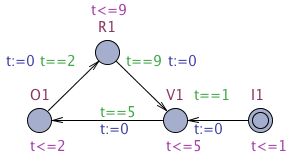
\includegraphics{ressources/part2/Q7-1.png}
	\caption{Automate du feu commençant en Vert}
\end{figure}

\begin{figure}[H]
	\centering
	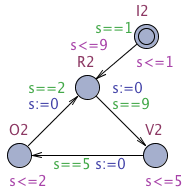
\includegraphics{ressources/part2/Q7-2.png}
	\caption{Automate du feu commençant en Rouge}
\end{figure}

%%%%%%%%%%%
\subsubsection{Validations}
%%%%%%%%%%%

\textbf{A n'importe quel moment il n'y a pas deux feux rouges en même temps}
\begin{verbatim}
A[](feu1.R1 or feu2.R2 or feu1.I1 or feu2.I2)
\end{verbatim}

\textbf{Pas de deadlock}
\begin{verbatim}
E<> deadlock
\end{verbatim}

%%%%%%%%%%%%%%%%%%%%%%%
\subsection{Question 8}
%%%%%%%%%%%%%%%%%%%%%%%

\href{https://github.com/masters-info-nantes/hong-cheng-lv/blob/master/ressources/part2/Q8-ControleurTemporiseEtSynchro.xml}{Un controleur temporisé est synchronisé avec les 2 feux pour changer leurs
états}

\begin{figure}[H]
	\centering
	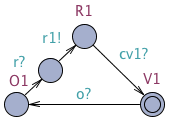
\includegraphics{ressources/part2/Q8-1.png}
	\caption{Automate du feu commençant en Vert}
\end{figure}

\begin{figure}[H]
	\centering
	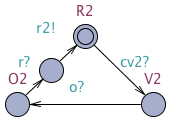
\includegraphics{ressources/part2/Q8-2.png}
	\caption{Automate du feu commençant en Rouge}
\end{figure}

\begin{figure}[H]
	\centering
	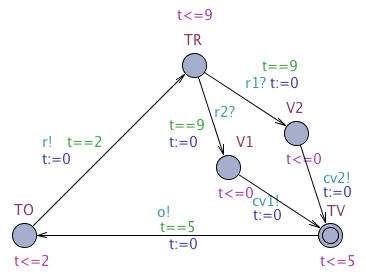
\includegraphics[width=1\textwidth]{ressources/part2/Q8-3.png}
	\caption{Contrôleur des feux}
\end{figure}

%%%%%%%%%%%
\subsubsection{Validations}
%%%%%%%%%%%

\textbf{A n'importe quel moment il n'y a pas deux feux rouges en même temps}
\begin{verbatim}
A[](feu1.R1 or feu2.R2)
\end{verbatim}

\textbf{?????????}
\begin{verbatim}
E<>(feu1.R1 and feu2.O2)
\end{verbatim}

\textbf{Pas de deadlock}
\begin{verbatim}
E<> deadlock
\end{verbatim}

%%%%%%%%%%%%%%%%%%%%%%%%%%%%%%%%%%%%%%%%%%%%
\section{Partie 3 - Carrefour en T}
%%%%%%%%%%%%%%%%%%%%%%%%%%%%%%%%%%%%%%%%%%%%

%%%%%%%%%%%%%%%%%%%%%%%
\subsection{Question 9}
%%%%%%%%%%%%%%%%%%%%%%%

\href{https://github.com/masters-info-nantes/hong-cheng-lv/blob/master/ressources/part3/Q9-SansContraintesTemps.xml}{Sans contraintes de temps}

\begin{itemize}
	\item 2 feux de la grande route considérés comme un seul
	\item Processus qui régule l'arrivée des voiture dans la petite rue
\end{itemize}

\begin{figure}[H]
	\centering
	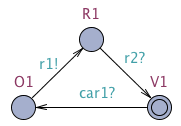
\includegraphics{ressources/part3/Q9-1.png}
	\caption{Automate du feu de la route majeure}
\end{figure}

\begin{figure}[H]
	\centering
	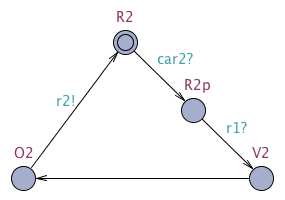
\includegraphics{ressources/part3/Q9-2.png}
	\caption{Automate du feu de la route mineure}
\end{figure}

\begin{figure}[H]
	\centering
	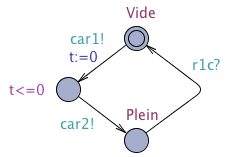
\includegraphics{ressources/part3/Q9-3.png}
	\caption{Automate de l'arrivée des véhicules sur la route mineure (capteur)}
\end{figure}

%%%%%%%%%%%%%%%%%%%%%%%
\subsection{Question 10}\label{question-10}
%%%%%%%%%%%%%%%%%%%%%%%

\href{https://github.com/masters-info-nantes/hong-cheng-lv/blob/master/ressources/part3/Q10-AvecContraintesTemps.xml}{Avec contraintes de temps}

\begin{itemize}
	\item Petite rue verte 30 secondes
	\item Dans un cycle, grande route verte au moins 30 secondes
	\item Delai de 1 seconde entre chaque changement de couleur
	\item Reste orange pendant 5 secondes
\end{itemize}

\begin{figure}[H]
	\centering
	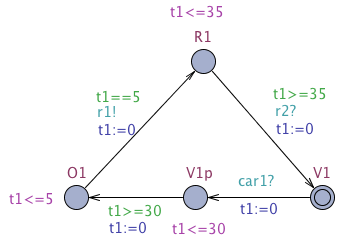
\includegraphics{ressources/part3/Q10-1.png}
	\caption{Automate du feu de la route majeure}
\end{figure}

\begin{figure}[H]
	\centering
	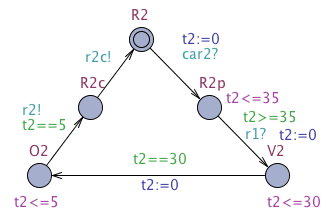
\includegraphics{ressources/part3/Q10-2.png}
	\caption{Automate du feu de la route mineure}
\end{figure}

\begin{figure}[H]
	\centering
	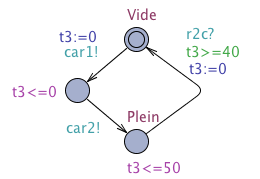
\includegraphics{ressources/part3/Q10-3.png}
	\caption{Automate de l'arrivée des véhicules sur la route mineure (capteur)}
\end{figure}

%%%%%%%%%%%%%%%%%%%%%%%
\subsection{Question 11}\label{question-11}
%%%%%%%%%%%%%%%%%%%%%%%

%%%%%%%%%%%
\subsubsection{Validations question 9}
%%%%%%%%%%%

\textbf{A n'importe quel moment il n'y a pas deux feux rouges en même temps}
\begin{verbatim}
A[](Major.R1 or Minor.R2 or Minor.R2p)
\end{verbatim}

\textbf{Pas de deadlock}
\begin{verbatim}
E<> deadlock
\end{verbatim}

%%%%%%%%%%%
\subdubsection{Validations question 10}
%%%%%%%%%%%

\textbf{A n'importe quel moment il n'y a pas deux feux rouges en même temps}
\begin{verbatim}
A[](Major.R1 or Minor.R2 or Minor.R2p)
\end{verbatim}

\textbf{Pas de deadlock}
\begin{verbatim}
E<> deadlock
\end{verbatim}

\end{document}
